\chapter{Implementation}

This chapter provides an overview of the important implementation details about the HaptiQ described in the Design chapter. 
Firstly, the hardware implementation is discussed, followed by the API. A dedicated section will discuss the tactons implementation. Finally, implementation details about applications will be covered.

\section{The Hardware}

Building the hardware components of the two HaptiQ devices has been a challenge on its own. Both the 4-HaptiQ and the 8-HaptiQ are 3D-modelled using Google Sketchup \todo[noline]{cite}. Models are then exported in the STL format, a standard in CAD software, and commissioned to a 3D printer. I used a MakerBot\textregistered   Replicator\texttrademark 2x. This is an experimental 3D printer, therefore high precision (\textless 2mm) is hard to achieve and requires many attempts before being able to print the wanted model. 

Phidgets boards are used to control the mini-servos and get pressure inputs. The wiring was more of a demanding task, rather than a challenging one.  

The different components of the device are assembled using super glue and screws (see the HaptiQ manual for more information on printing and assembling). 

\subsection{Fiducial Markers}

The provided API supports the recognition of two types of fiducial markers: Microsoft Bytetags and GRATF Glyphs. The HaptiQs built for this project place the fiducial markers on the bottom side. However, the GRATF Glyphs can also be placed on top the device, assuming that an appropriate structure around the HaptiQ is built, and can be recognised using a simple web-cam.  

\begin{figure}
        \centering
        \begin{subfigure}[H]{0.3\textwidth}
                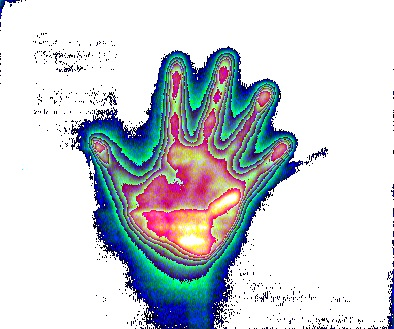
\includegraphics[width=\textwidth,height=\textwidth]{hand.jpg}
                \caption{Raw image of Hand}
                \label{fig:rawHand}
        \end{subfigure}%
        ~ %add desired spacing between images, e. g. ~, \quad, \qquad etc.
          %(or a blank line to force the subfigure onto a new line)
        \begin{subfigure}[H]{0.3\textwidth}
                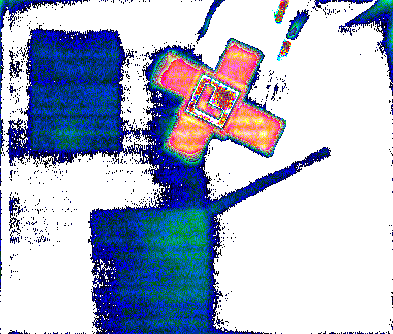
\includegraphics[width=\textwidth,height=\textwidth]{type1.png}
                \caption{Raw image of 4-HaptiQ with Glyph - type 1}
                \label{fig:rawHaptiQ1}
        \end{subfigure}
        ~ %add desired spacing between images, e. g. ~, \quad, \qquad etc.
          %(or a blank line to force the subfigure onto a new line)
        \begin{subfigure}[H]{0.3\textwidth}
                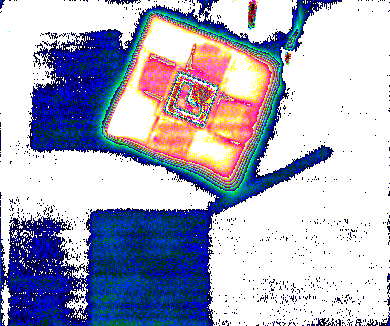
\includegraphics[width=\textwidth,height=\textwidth]{type2.png}
                \caption{Raw image of 4-HaptiQ with Glyph - type 2}
                \label{fig:rawHaptiQ2}
        \end{subfigure}
        \caption{Raw images}\label{fig:rawImages}
\end{figure}

The Bytetags, according to Microsoft, can be printed on normal office paper \footnote{http://msdn.microsoft.com/en-us/library/ee804862(v=surface.10).aspx}. However, during the first implementation phase of this project it has been evident that printed Bytetags lead to poor results, with the fiducial markers being tracked at low frequency.

The alternative solution is to use glyphs. The Surface SDK 2.0 allows to retrieve raw image data from the interactive table. Having access to this data, it is possible to apply common image matching algorithms to identify particular objects. This is achieved using GRATF, a C\# library that allows recognition and localization of glyphs in still images. 

Figure ~\ref{fig:rawImages} shows three raw images retrieved through the Surface SDK 2.0. The Microsoft PixelSense uses near-infrared sensors. So the Figure ~\ref{fig:rawHand}, for instance, represents how the hand absorbs infrared light, rather than its heat values as one may think. Glyphs are $n \times n$ grids, with n from 5 to 8, where each cell is either black or white (see Figure  ~\ref{fig:glyph}) and minimum side length of 8mm, that can be printed using Glyph Recognition Studio \footnote{Available at http://www.aforgenet.com/projects/gratf/}. Additional rules apply, such that that the border cells can only be white and the glyph cannot be symmetrical in any of its axis. The base of the HaptiQ is covered with white paper, so that the black tiles in the glyphs are recognised more easily (see Figure ~\ref{fig:rawHaptiQ1}). However, this is not sufficient for the glyph to be recognised at all angles. After testing glyphs of different dimensions and on different surfaces, I found out that extending the glyph with low absorption material (e.g. white foam board) improves the recognition of the glyph significantly (see Figures ~\ref{fig:rawHaptiQ2} and ~\ref{fig:whitesurface}).   

\begin{figure}[H]
  \centering
  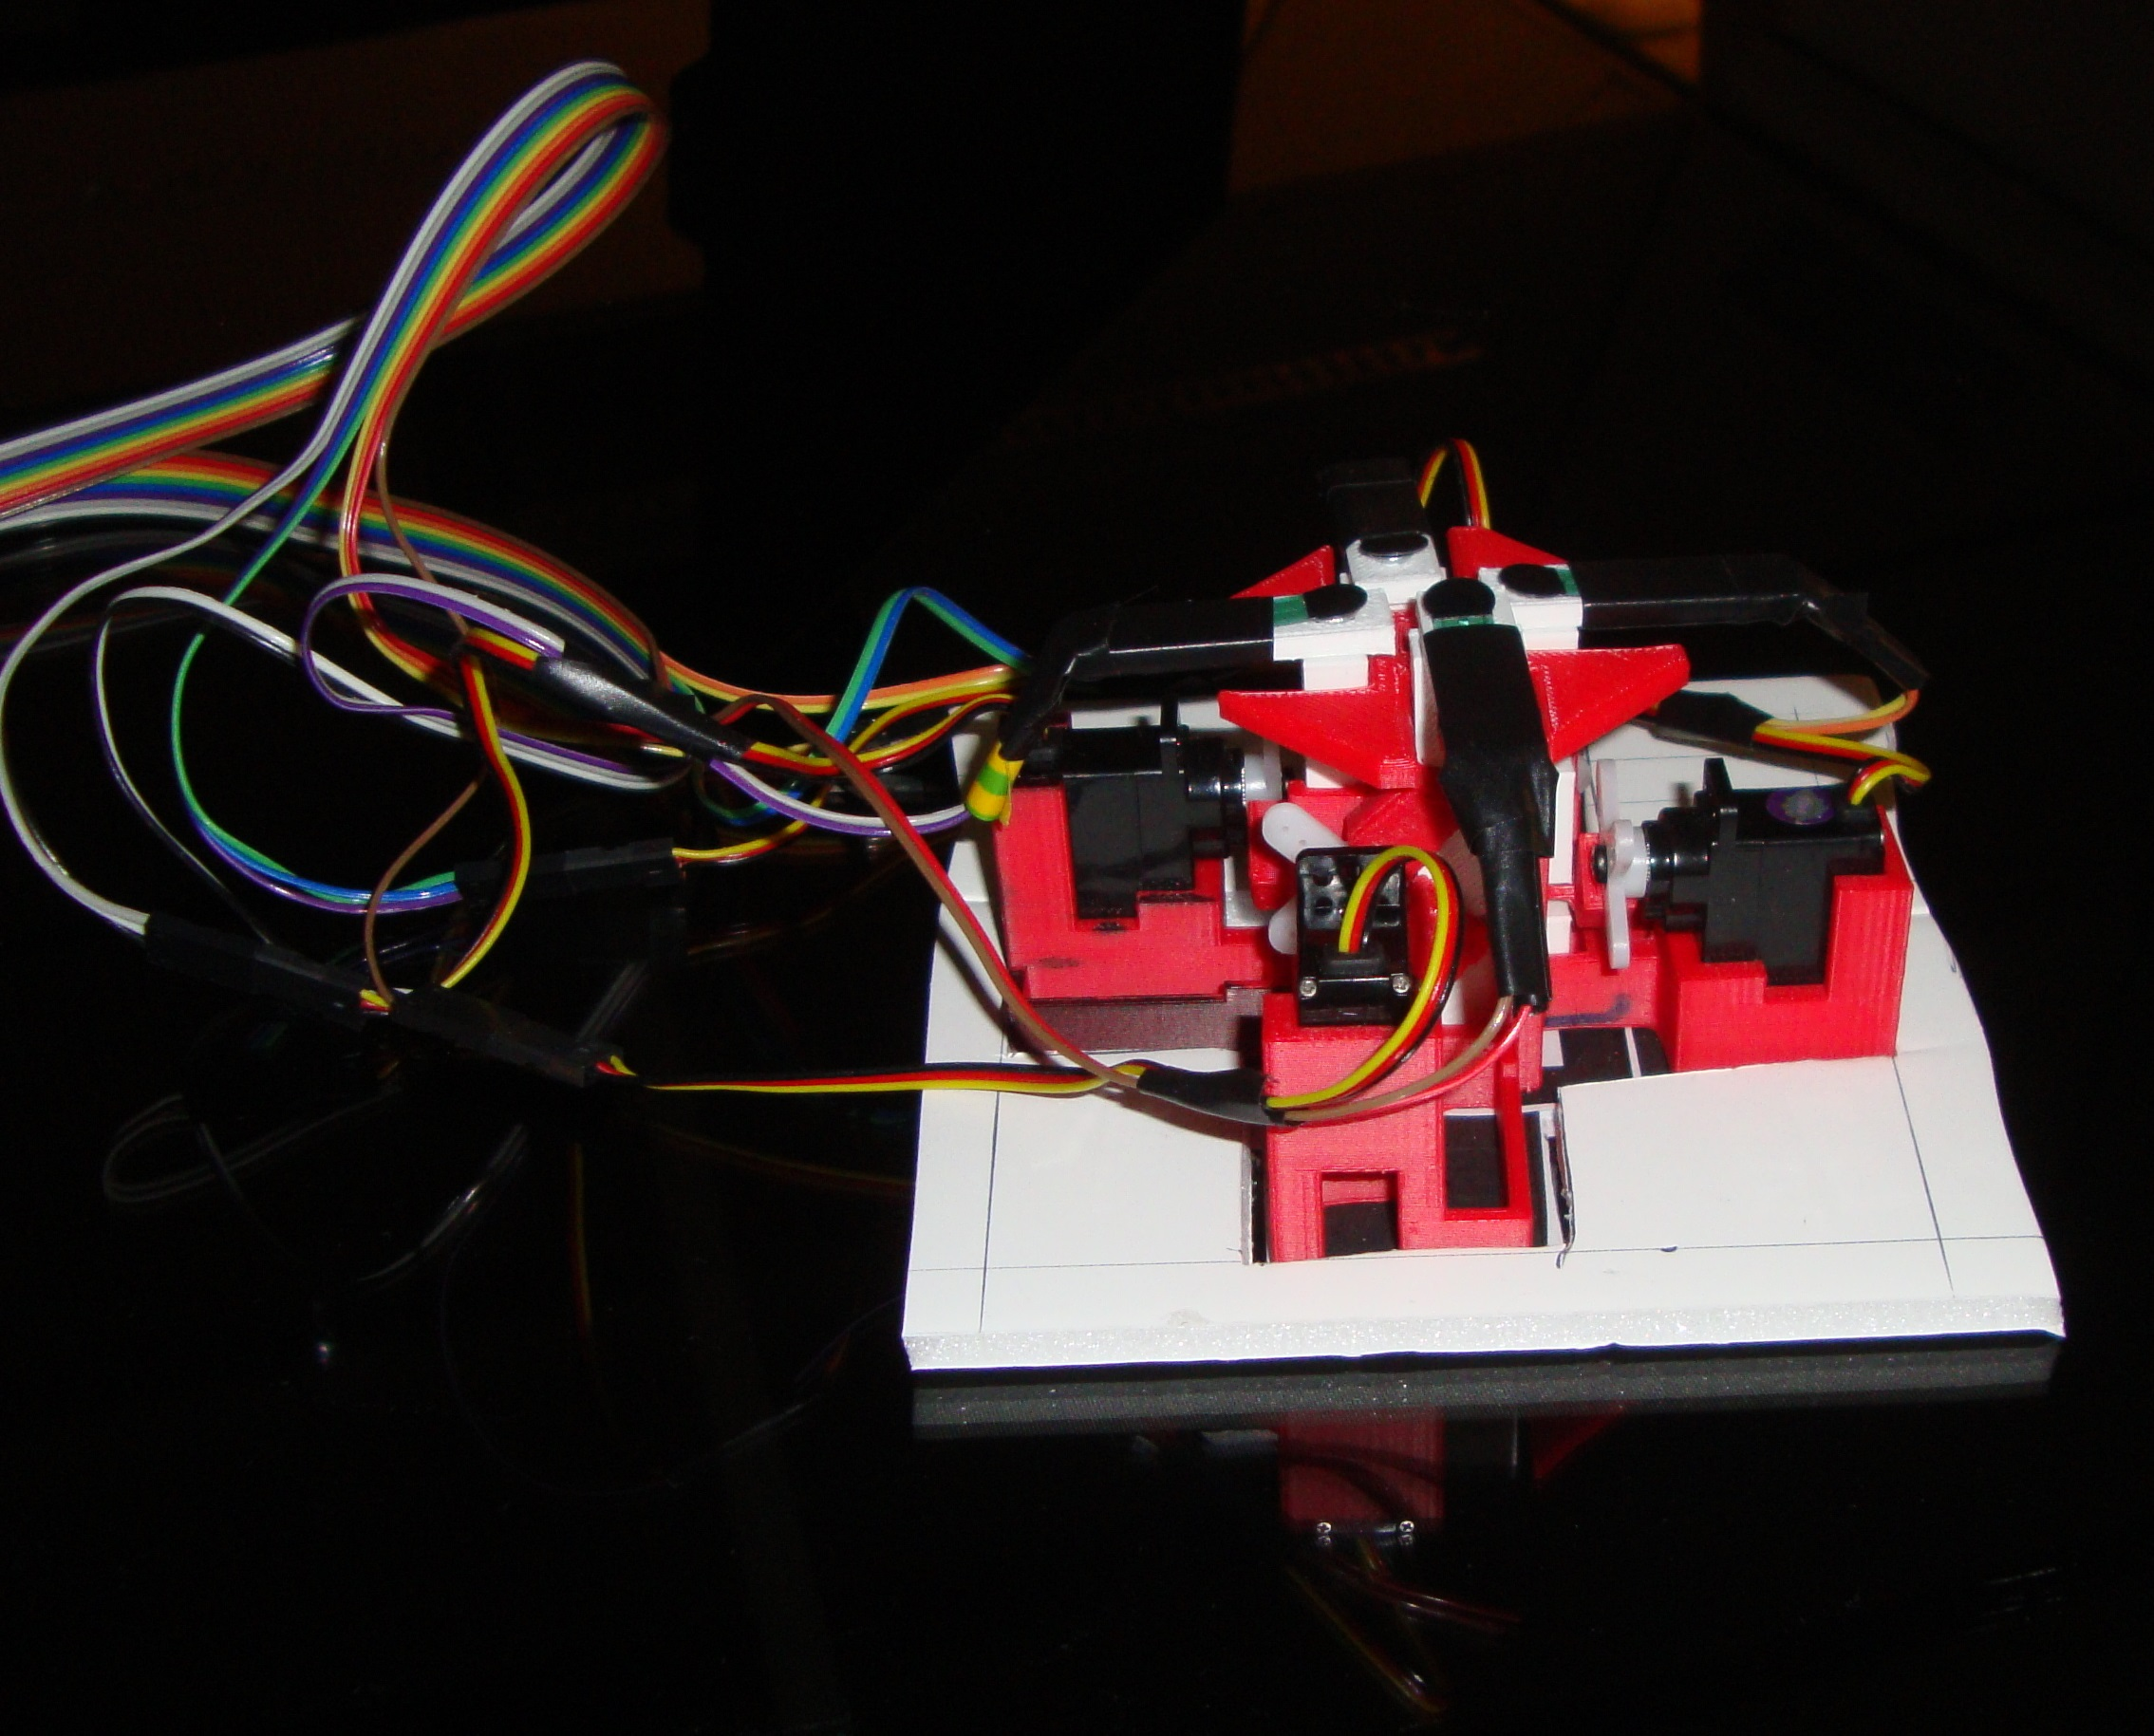
\includegraphics[width=0.5\textwidth]{DSC06783.JPG}
  \caption{HaptiQ with extended white board base}
  \label{fig:whitesurface}
\end{figure}

\section{The API}

\subsection{Input API}

The Input API is the component used to retrieve the HaptiQ location on the tabletop. It follows that this is highly hardware dependent on the used hardware. The current targeted hardware is the Microsoft Tabletops using the Surface SDK 2.0. Code to retrieve image data from web-cams is also provided. 
As explained in the design section, two main classes exist in the Input API: one to recognise Bytetags and one to recognise glyphs. The Bytetags currently places on the interactive table are easily recognised using the \textit{TouchTarget} object of the \textit{Microsoft.Surface.Core} library. On the other hand, glyphs are recognised by calling the \textit{FindGlyphs} function, from the GRATF library, on a bitmap image. GRATF does not provide any functionality to estimate the position and the rotation of the glyphs. When a glyph is recognised, all its vertices are known. The position is estimated by calculating the crossing point between the two diagonals of the glyph. The rotation, instead, is estimated using the inclination angle of one of the edges of the glyph. 

The API raises events of the form:
\lstset{style=sharpc1}
\begin{lstlisting}
delegate void ChangedEventHandler(object sender, InputIdentifier inputIdentifier, Point point, double orientation, EventArgs e);
\end{lstlisting}

in order to notify the current location of a device, recognisable by a unique identifier (Bytetag or glyph). Then the HaptiQsManager, from within the HaptiQ API, handles such events.  

\subsection{HaptiQ API}

\todo[inline, color=green!40]{discuss implementation details of the HaptiQ API such as multithreading}

\subsubsection{Haptic Objects}

describe input handling, multiple device handling, states change etc

\subsection{Examples}

In this section, I will show how to use the API using a simple example (see Code ~\ref{lst:basicAPIUsage}). This section is necessary to properly understand section ~\ref{sec:Applications}, which discusses the provided example applications of this project.

The first step consists in creating a WPF application and add a reference to the HaptiQ\_API. From the code view of the application, import the HaptiQ\_API and the HapticClientAPI namespaces (the latter contains the default HapticObjects). 

The call \textit{HaptiQsManager.Create(windowTitle, "\textless Input Class\textgreater")} initialises the HaptiQ device and the Input API, using the specified Input class (e.g. "SurfaceInput" for Bytetags). 
Objects are automatically added to the system when they are created. These are rendered only when added to a WPF grid or canvas. 
The call \textit{HaptiQsManager.Instance.delete()} ensures that the HaptiQs are detached correctly and all resources are disposed correctly.

\lstset{style=sharpc}
\begin{lstlisting}[caption={Basic API usage},label={lst:basicAPIUsage}]
using HaptiQ_API;
using HapticClientAPI;

public partial class Application : SurfaceWindow
{
  public Application()
  {
      HaptiQsManager.Create(windowTitle, "SurfaceInput");
      
      HapticShape rect0 = new HapticRectangle(50, 50, 150, 200);
      rect0.color(Brushes.Salmon);
      this.container.Children.Add(rect0);
      
      HapticShape rect1 = new HapticRectangle(150, 350, 200, 200);
      rect1.color(Brushes.Orange);
      this.container.Children.Add(rect1);
      
      HapticShape rect2 = new HapticRectangle(550, 150, 100, 100);
      rect2.color(Brushes.Green);
      this.container.Children.Add(rect2);
      
      HapticShape link = new HapticLink(rect2, rect1);
      link.color(Brushes.White);
      this.container.Children.Add(link);
  }
  
  protected override void OnClosed(EventArgs e)
  {
      base.OnClosed(e);
      HaptiQsManager.Instance.delete();
      Application.Current.Shutdown();
  }
}
\end{lstlisting}

\todo[inline, color=green!40]{add image of the resulting application}

Please refer to the HaptiQ manual for additional examples on how to use the API. 

\section{Configuration}

\begin{itemize}
\item Use windows forms.
\item pop up until there are phidget boards to be configured
\end{itemize}

\section{Tactons}

\begin{itemize}
\item explain initial approach
\item explain generalised approach using bitwise operations
\end{itemize}

\lstset{style=sharpc1}
\begin{lstlisting}[caption={Tactons - Initial approach},label={lst:basicAPIUsage}]
private int[][][] directionMatrix = new int[][][]
                    {  new int[][]{                 // vertical 
                        new int[]{0, 1, 0, 1, 0}, 
                        new int[]{1, 1, 1, 0, 0}, 
                        new int[]{0, 0, 1, 0, 1}, 
                        new int[]{1, 1, 0, 0, 1}, 
                        new int[]{0, 1, 0, 1, 0}, 
                        new int[]{1, 1, 1, 0, 0}, 
                        new int[]{0, 0, 1, 0, 1}, 
                        new int[]{1, 1, 0, 0, 1}}, 
                    new int[][]{                    // horizontal
                        new int[]{0, 0, 1, 0, 1},
                        new int[]{1, 1, 0, 0, 1},
                        new int[]{0, 1, 0, 1, 0},
                        new int[]{1, 1, 1, 0, 0},
                        new int[]{0, 0, 1, 0, 1},
                        new int[]{1, 1, 0, 0, 1},
                        new int[]{0, 1, 0, 1, 0},
                        new int[]{1, 1, 1, 0, 0}},
                   ...
                   };
\end{lstlisting}

\section{Applications}
\label{sec:Applications}

This section will briefly explain some of the implementation details about the two example applications provided with this project.

\subsection{Graph Visualisation}

\subsection{Functions Visualisation}

\begin{itemize}
\item use of NCalc \footnote{http://ncalc.codeplex.com/} for evaluating inpu tmathematical expression
\item scaling functions
\end{itemize}



